\chapter{Tiny trainable instruments}

\epigraph{All the modern things \\ have always existed \\ they've just been waiting}{The Modern Things \\ Björk, 1995}

This chapter describes the process of conceptualizing and developing this antidisciplinary thesis project, drawing from the fields of \acrlong{AI}, electrical engineering, computer science, media arts, music, and pedagogy, among others.

First, let me explain my definitions of the words that make up the title of this project.

\section{Definition of Tiny trainable instruments}

\subsection{Definition of tiny}

By \emph{tiny} I mean lightweight handheld instruments, that you can fit on a backpack, or take for a walk. This is inspired on my personal practice: for years I have accumulated many small tools for arts that I perform gigs with, or that I carry with me while traveling, mostly small electronic synthesizers, sound mixers, and battery-powered speakers.

Here is an example of a yellow handheld sampler with an included microphone and speaker that I enjoy for field recordings, and with a green battery pack for portability.

\begin{figure}[ht]
  \centering
  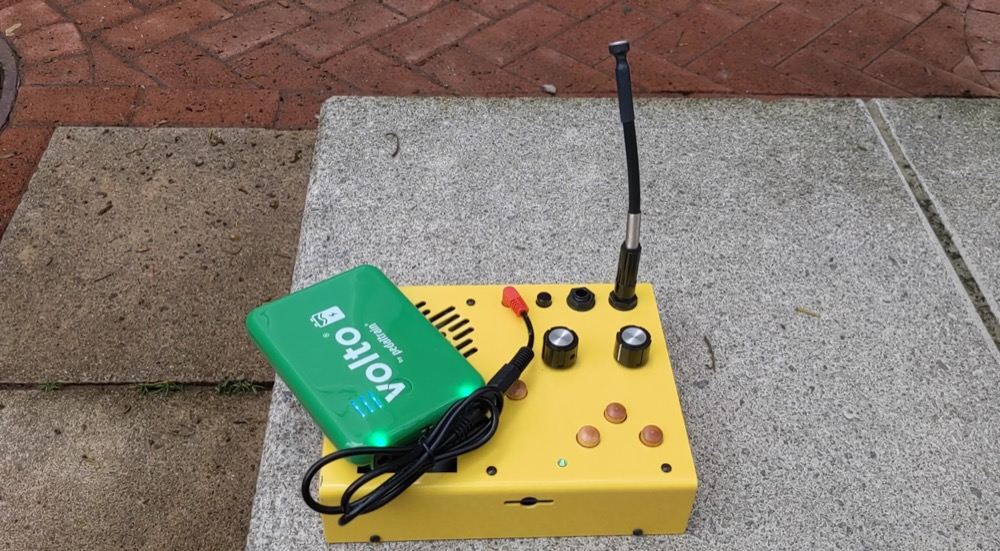
\includegraphics[width=0.75\linewidth,height=0.25\textheight,keepaspectratio]{images/critter-and-guitari-kaleidoloop-battery.jpg}
  \caption{Sampler with microphone and portable battery}
  \caption*{Picture taken by myself}
  \label{fig:critter-and-guitari-kaleidoloop-battery}
\end{figure}

\emph{Tiny} is also a nod to the emerging field and community of tiny \acrshort{ML}, including most importantly for me the tinyMLx professional certificate\cite{website-edx-harvardx-tinymlx-professional-certificate} offered by HarvardX, that I completed while working on this project.

With that, the \emph{tiny} in \emph{Tiny trainable instruments} comes from them being handheld on an breadboard, for being able to be powered from a generic USB power bank, and for using tiny \acrshort{ML} for mediating their inputs and outputs.

\subsection{Definition of trainable}

By \emph{trainable} I mean a device that can learn by examples. This name comes from the \acrshort{ML} lexicon, where training is a process where an algorithm  iteratively finds the numerical values of all parameters (weights, biases) of a \acrshort{ML} model.

Training a device is particularly attractive for artists working with sensors. The Arduino microcontroller that this thesis uses has several embedded sensors, which we can use to produce huge streams of data, like this screenshot of it outputting raw data from its \acrshort{RGB} sensor for color.

\begin{figure}[ht]
  \centering
  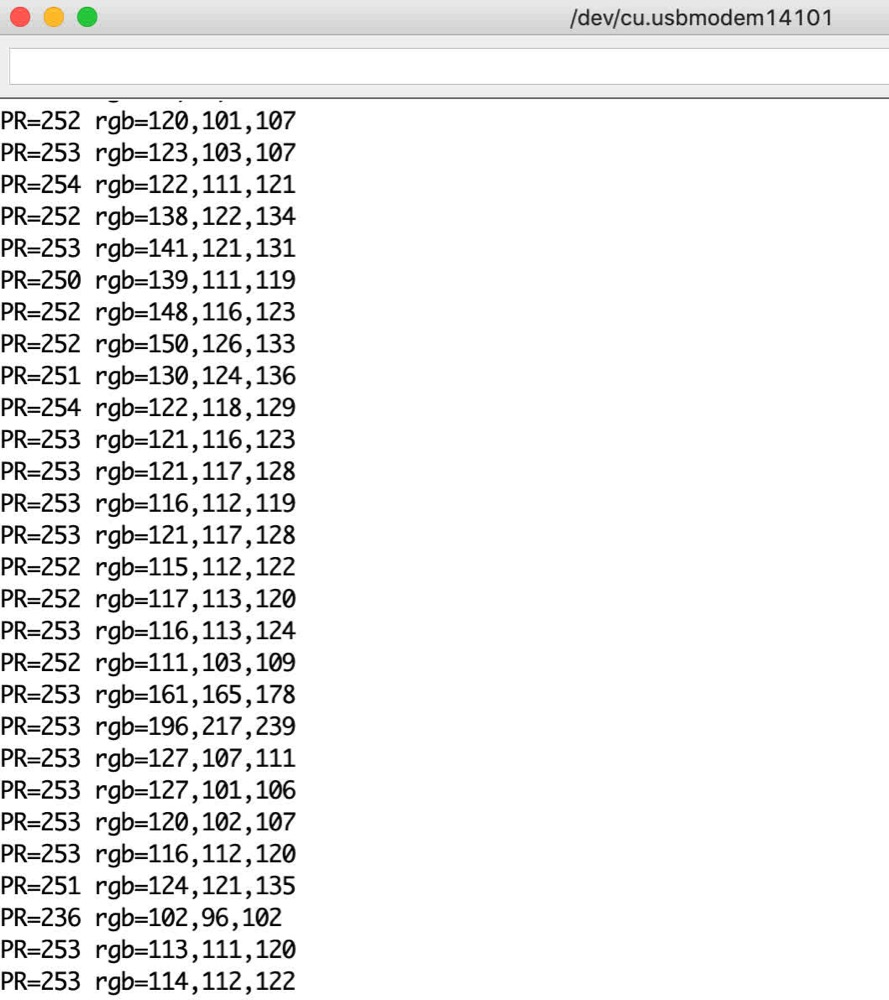
\includegraphics[width=0.75\linewidth,height=0.40\textheight,keepaspectratio]{images/arduino-data-stream.jpg}
  \caption{Data stream from embedded sensors in an Arduino microcontroller}
  \caption*{Screen capture by myself}
  \label{fig:arduino-data-stream}
\end{figure}

If we wanted to use this sensor at home to detect a red object, we can start by taking notes of the \acrshort{RGB} values of the sensor when the red object is close to it, and then include this value as a threshold for detection on the software uploaded to the microcontroller. Since the \acrshort{RGB} sensor needs a consistent lighting, we need to be really careful with the lighting conditions, and if they change, we have to look at the stream of data to find the new value for red, and update the code, and reprogram the microcontroller.

This is a tedious process, and it inspired me to work on this thesis, so that I could help artists use \acrshort{ML} and microcontrollers to capture data, then train a model, and let the algorithm figure out the correct answer, without having to write more code!

An educational and creative example I recommend checking out is Teachable Machine by Google \cite{website-google-teachable-machine}, a web application that allows you to use your computer's microphone and webcam to generate data, and then train models that can detect different words, images, or body postures, without having to write any line of code.

In particular, I became interested on tiny \acrshort{ML} examples that requires small databases, and that can be trained on device, for the use case of making an instrument that you can change its behavior mid performance, like guitar players do with their guitars, when they change their tunings between songs. With my thesis you can program a device that can detect an apple, and then five minutes later, an orange, and then for your last song, a grapefruit. Hat tip to Sonic Youth, a band that used to tour with more than a dozen guitars, each one of them with a different tuning, and they would switch instruments between songs.

\begin{figure}[ht]
  \centering
  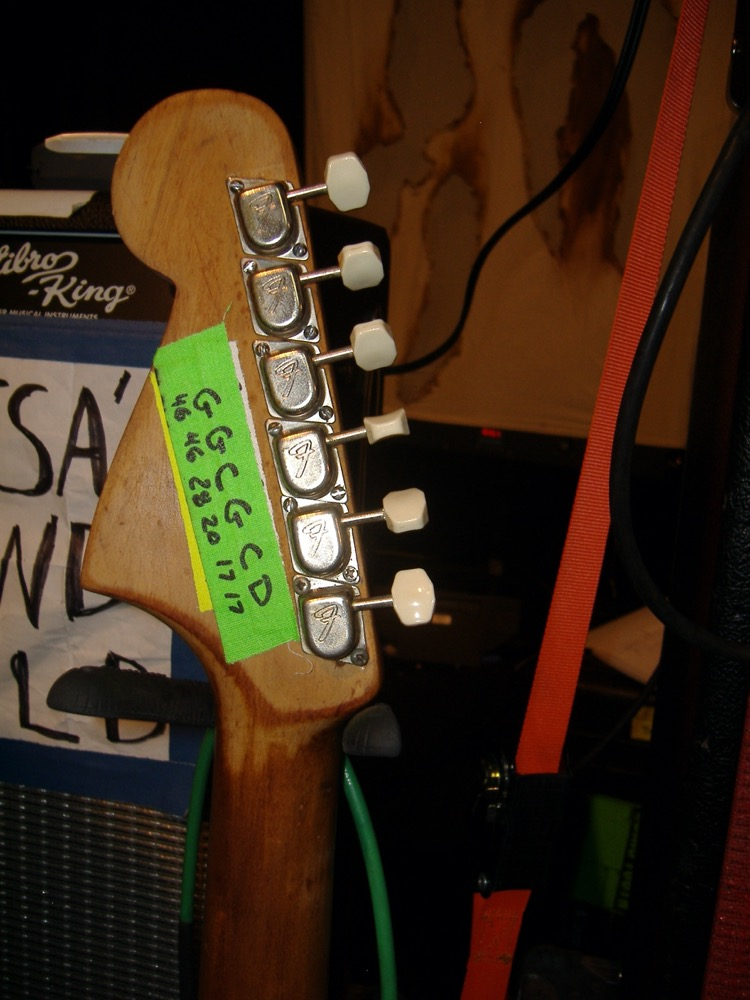
\includegraphics[width=0.75\linewidth,height=0.30\textheight,keepaspectratio]{images/sonic-youth-guitar.jpg}
  \caption{Sonic Youth guitar with custom tunings}
  \caption*{Retrieved from \cite{sonic-youth-illustrated-equipment-guide}}
  \label{fig:sonic-youth-guitar}
\end{figure}

\subsection{Definition of instruments}

By \emph{instruments} I mean devices that transduce energy across different media. Instruments receive an input, process it, and then produce an output. For musical instruments I like to think about instruments are able to not just produce musical notes from western scales, but a wide spectrum of sounds, encompassing the wide vocabulary of experimental electronic music and electroacoustic music.

On top of that, my personal definition of \emph{instrument}, includes having freedom and liberty, no censorship. This is why I consider my bicycle to be an art instrument, that transduces my pedalling input into multimedia output: adventure, sweat, and wind in my face. Also, while I am riding it I am not subjected to the restrictions of any corporate or government playground, there are mostly no rules besides gravity, and there are no backdoors that anyone can use to track me, exploit me, or limit my speed (we have smartphones for corporate and government surveillance, but that's another story).

The liberties that \emph{instruments} make me feel, are a huge contrast to the computational tools I am using for crafting this thesis. I am typing on an Apple Macbook, and even though I like its keyboard and portability, I am aware that I face restrictions: Apple wants developers to pay to be certified developers, and if I update my operating system I won't be able to run 32 bits apps anymore. This thesis is hosted on GitHub, which is a service blocked for developers in certain countries due to USA sanctions \cite{website-github-trade-controls}. I am from a country recently affected by a dictatorship and human rights violations, and some of my relatives have been exiled, so I am particularly sensitive to policies that limit people's freedom of speech and computing.

This uncomfort also was a catalyst for the creation of \textit{Tiny trainable instruments}, which are based on open source off-the-cloud microcontrollers, and nobody can censor me when I use them for arts, thus being \emph{instruments}, as gratifying as playing with my guitar and bicycle, and I hope you feel that joy too while on this thesis.

\section{Components of the project}

In this chapter I will explain both the process and the result of each component of this thesis:

\begin{enumerate}
  \item TinyTrainable Arduino software library
  \item Code for training \acrshort{ML} with \acrshort{DIY} databases
  \item Workshop and educational material
\end{enumerate}

\subsection{TinyTrainable Arduino software library}

This project's main contribution is the TinyTrainable Arduino software library, which allows you to create flexible multimedia instruments, where you can combine any input with any output, and it runs on the microntroller Arduino Nano 33 BLE Sense. This microcontroller was chosen because it is currently the only Arduino supported by the Arduino Tensor Flow Lite library.

\begin{figure}[ht]
  \centering
  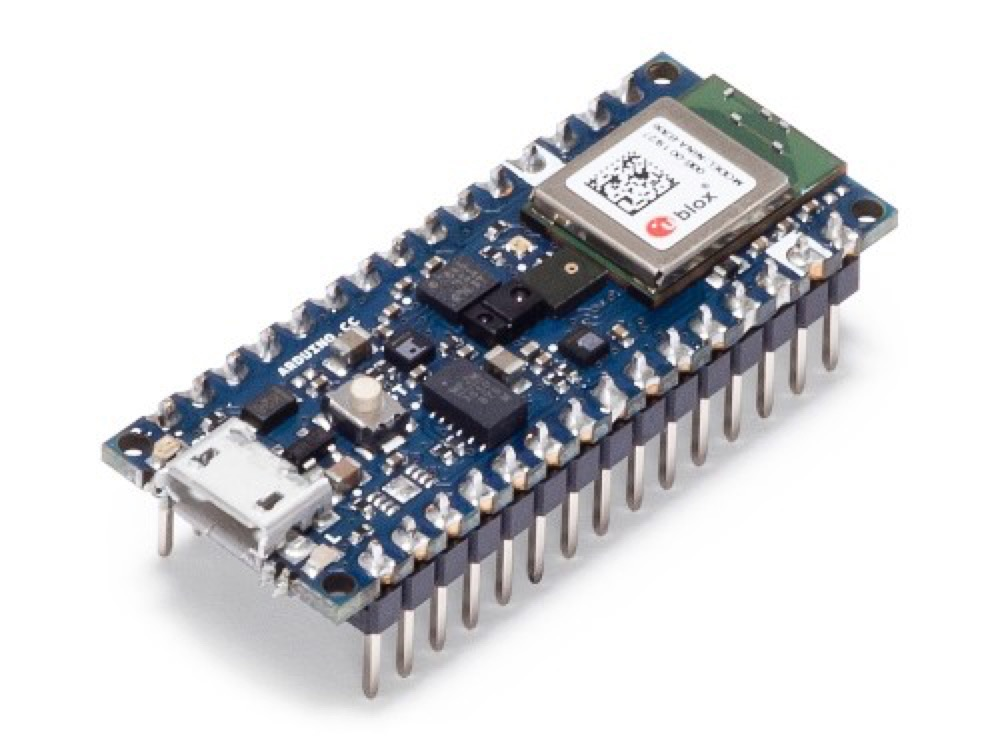
\includegraphics[width=0.75\linewidth,height=0.30\textheight,keepaspectratio]{images/materials-arduino-nano-33-ble-sense.jpg}
  \caption{Arduino Nano 33 \acrshort{BLE} Sense microcontroller with headers}
  \caption*{Retrieved from \cite{website-materials-arduino-nano-33-ble-sense}}
  \label{fig:materials-arduino-nano-33-ble-sense}
\end{figure}

The TinyTrainable library is flexible, since it allows us to combine any of the 3 available inputs, with any of the 7 possible outputs, summarized on this table, for a total of 21 possibilities!

\begin{table}[ht]
    \centering
    \begin{tabular}{ | l | l | l | l | l | l | l | l |}
        \hline
        \textbf{\backslashbox{Input}{Output}}  & Buzzer & \acrshort{LED} & \acrshort{MIDI} & Printer & Screen & Serial & Servo \\
        \hline
        Color & & & & & & & \\
        \hline
        Gesture & & & & & & & \\
        \hline
        Speech & & & & & & & \\
        \hline
    \end{tabular}
    \caption{Matrix of inputs and outputs}
    \label{table:tiny-trainable-instruments-inputs-outputs-matrix}
\end{table}{}

For the inputs I used the embedded sensors of the Arduino microcontroller with their corresponding open source libraries, and processed the input data with 2 recently released open source \acrshort{ML} libraries, summarized on this table.

\begin{table}[ht]
    \centering
    \begin{tabular}{ | l | l | l |}
        \hline
        \textbf{Input}  & \textbf{Sensor library} & \textbf{\acrshort{ML} library} \\
        \hline
        Color &  Arduino{\_}APDS9960 & Arduino{\_}KNN \\
        \hline
        Gesture & Arduino{\_}LSM9DS1 & Arduino{\_}TensorFlowLite \\
        \hline
        Speech & PDM & Arduino{\_}TensorFlowLite \\
        \hline
    \end{tabular}
    \caption{Software dependencies for inputs}
    \label{table:software-dependencies-inputs}
\end{table}{}

The outputs rely on extra hardware, and in some cases, external libraries, which are summarized here.

\begin{table}[ht]
    \centering
    \begin{tabular}{ | l | l | }
        \hline
        \textbf{Output}  & \textbf{Actuator library} \\
        \hline
        Buzzer & - \\
        \hline
        \acrshort{LED} & - \\
        \hline
        \acrshort{MIDI} & - \\
        \hline
        Printer & Adafruit Thermal Printer Library\\
        \hline
        Screen & Adafruit{\_}SSD1306\\ 
        \hline
        Serial & - \\
        \hline
        Servo & Servo\\
        \hline
    \end{tabular}
    \caption{Software dependencies for outputs}
    \label{software-dependencies-outputs}
\end{table}{}

\subsubsection{Repository structure}

The TinyTrainable library is a repository hosted at \url{https://github.com/montoyamoraga/TinyTrainable}, where you can review all the history and commits through time, where anyone can see how the library or each file has evolved over time.

The structure of the folders follows 2 simultaneous specifications: it includes the necessary file and folder names for being packaged and indexed as an Arduino Library, and on top of that it complies with GitHub guidelines for licensing libraries, and for automatic workflows for code testing.

The source code of the library is written in C++ and is located in the src/ folder. The examples live in the examples/ folder, and are written in the Arduino langauge. The examples are divided in 4 folders: 1 for each input, and 1 extra for checking the wiring of each output.

Some trained \acrshort{ML} models are included as C++ files on the assets/ folder. 

\subsubsection{Installation}

The library can be downloaded from the Releases section of the repository at  \url{https://github.com/montoyamoraga/TinyTrainable/releases}, where you also have access to the complete history of releases over time. To install it, you need to uncompress the .zip into a folder, and then make it discoverable by the Arduino IDE.

Since that method is not automatic and could be prone to errors, I made the effort to publish the TinyTrainable library, by complying with the latest Arduino Library Manager specifications, detailed on their repository \url{https://github.com/arduino/library-registry/}. With that, from the Arduino IDE you can open their Library Manager and do a 1 click installation of the library, or as an alternative use arduino-cli, the Arduino command line tool on your terminal.

\subsubsection{Hardware basics}

The TinyTrainable library has only 1 fixed and particular hardware requirement: it only runs on the Arduino Nano 33 \acrshort{BLE} Sense, a microcontroller released in 2019. For powering it you need a generic micro USB cable to provide the necessary input of 5V. To upload code to the microcontroller you can use the same USB cable to connect to a computer running the Arduino IDE.

\begin{figure}[ht]
  \centering
  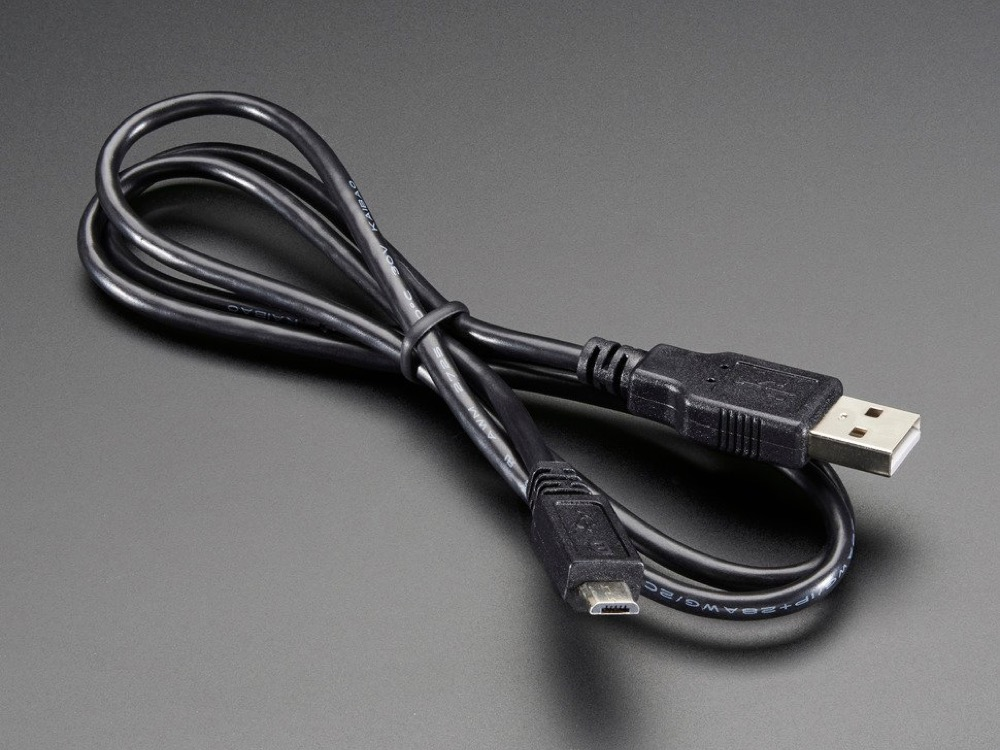
\includegraphics[width=0.75\linewidth,height=0.25\textheight,keepaspectratio]{images/materials-adafruit-micro-usb-cable.jpg}
  \caption{Micro USB cable}
  \caption*{Retrieved from \cite{website-materials-adafruit-micro-usb-cable}}
  \label{fig:materials-adafruit-usb-cable}
\end{figure}

To build a Tiny trainable instrument, you also need a breadboard, jumper wires, and one of the many possible output devices that I will describe soon.

\begin{figure}[ht]
  \centering
  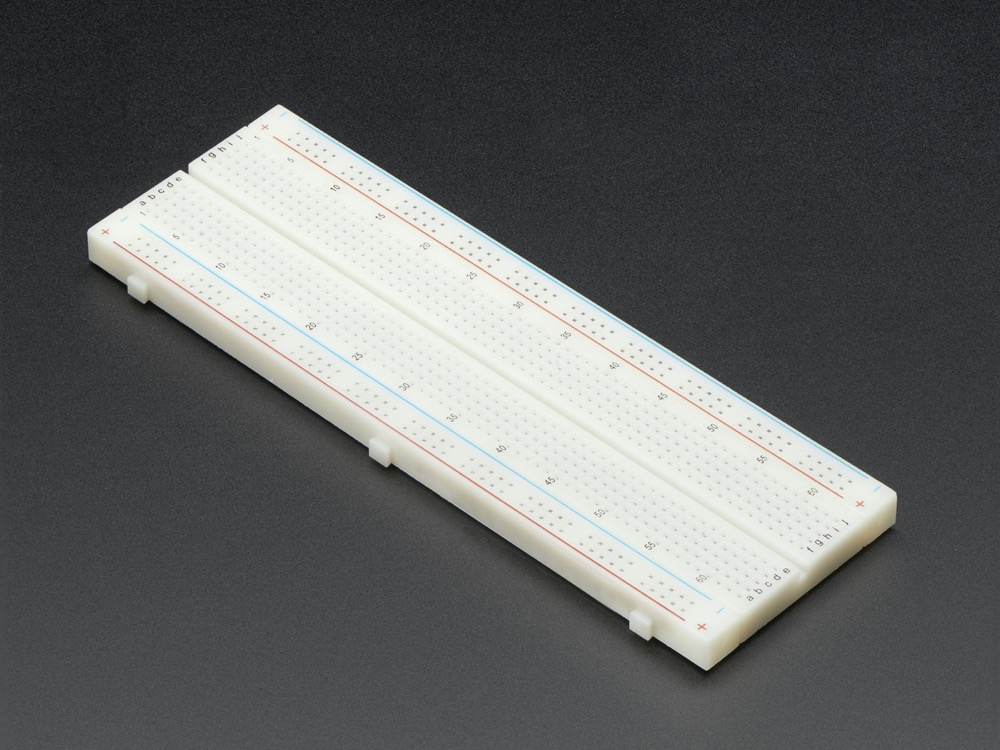
\includegraphics[width=0.75\linewidth,height=0.25\textheight,keepaspectratio]{images/materials-adafruit-breadboard.jpg}
  \caption{Breadboard}
  \caption*{Retrieved from \cite{website-materials-adafruit-breadboard}}
  \label{fig:materials-adafruit-breadboard}
\end{figure}

\begin{figure}[ht]
  \centering
  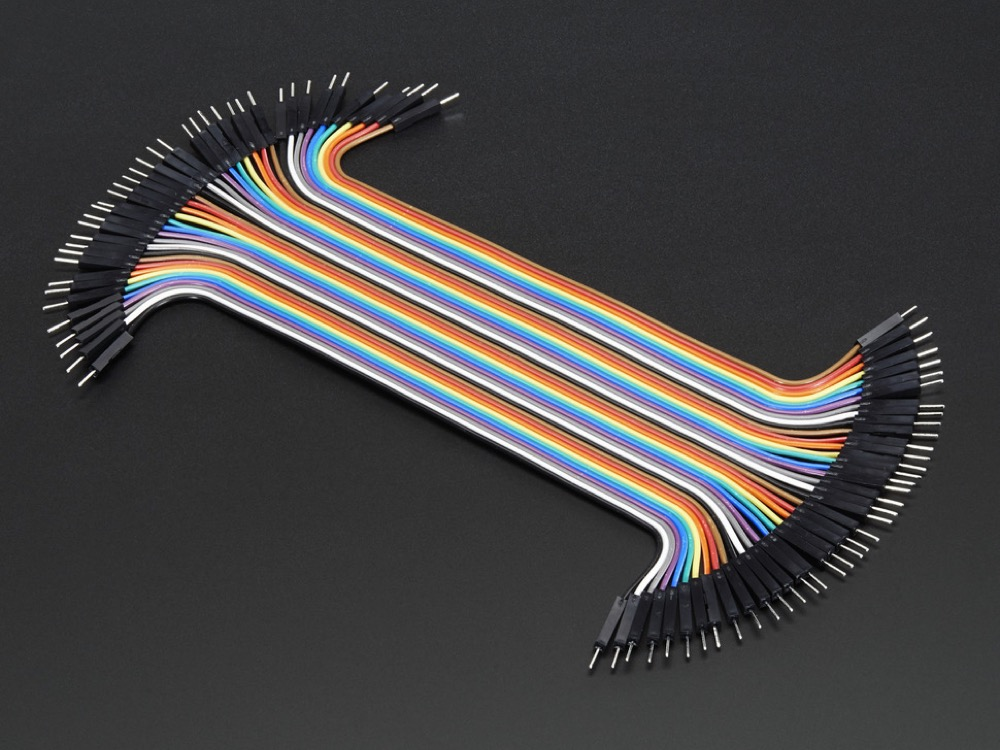
\includegraphics[width=0.75\linewidth,height=0.25\textheight,keepaspectratio]{images/materials-adafruit-jumper-wires.jpg}
  \caption{Jumper wires}
  \caption*{Retrieved from \cite{website-materials-adafruit-jumper-wires}}
  \label{fig:materials-adafruit-jumper-wires}
\end{figure}

Let's now dive deep into the different inputs and outputs for building a Tiny trainable instrument.

\section{Inputs}

As I mentioned before, for the inputs no extra wiring is needed, since we are using the embedded sensors of the Arduino microcontroller, to detect the 3 possible inputs: color, gesture, and speech. These inputs were designed to foster different behaviors with the library, which are detailed in the following sections.

In terms of software, there is a base class Input on the source code, which stores common properties and methods for all inputs, and this class is inherited to each of the different inputs.

\subsection{Color input}

The color input allows artists to build Tiny trainable instruments that can detect the color of objects near to the microcontroller. I recommend that this is the first input that people try, since it is the easiest to implement, and the fastest to use.

For detecting color, the TinyTrainable is a wrapper of the Arduino{\_}APDS9960 library, needed to access the data of the embedded distance and color sensor of the microcontroller. This allows the instrument to detect nearby objects, and when they are close enough to the microcontroller, it reads a 1 pixel \acrshort{RGB} value, detecting how red, how green, and how blue any object is.


It accomplishes this feat by relying on 2 software libraries:  for the sensor, and Arduino{\_}KNN for \acrshort{ML}. For the color reading, the sensor first detects distance of objects near the Arduino microcontroller, 

\subsection{Gesture input}

The gesture input allows artists to build Tiny Trainable instruments that can detect different motion gestures, by moving the microcontroller in space.

\subsection{Speech input}

The speech input allows artists to build Tiny Trainable instruments that can detect different sounds or utterances, by emitting sound next to the microcontroller.

\section{Design principles}

\begin{enumerate}
  \item Affordable
  \item Hackable
  \item Open
  \item Private
\end{enumerate}

\subsection{Cheap}

The materials for this thesis 

\section{Open}

All examples included with this library were written with the aim of showing the fundamentals of how to build the instruments and different \acrshort{ML} enabled manipulation of multimedia material, so that people could build on top of it and make it their own, by changing the values of variables and adding more functionalities.

\section{Philosophy and experience}

Throughout this project, the magic number was 3. The \acrshort{ML} algorithms were hardcoded to be able to distinguish between 3 different categories: 3 colors, 3 physical gestures, 3 sound utterances.


\subsection{Color}

This approach uses the \acrshort{RGB} color sensor from the microcontroller, with the auxiliary help from the proximity sensor, that is used to capture color information at a certain distance threshold.

The data is passed to a k-Nearest-Neighbor algorithm, programmed using the Arduino KNN library.

\subsection{Gesture}

This input uses the information from the Inertial Measurement Unit (IMU) of the microcontroller, including a gyroscope and accelerometer. It captures data after a certain threshold of movement is detected.

The data is passed to a TensorFlow neural network, programmed using the Arduino TensorFlow Lite library, and based on the included magic$\_$wand example.

\subsection{Speech}

This input uses the information from the microphone of the microcontroller.

The data is passed to a TensorFlow neural network, programmed using the Arduino TensorFlow Lite library, and based on the included micro$\_$speech example.

\section{Outputs}

The different outputs were picked, because of their low cost, ubiquity, and possibilities of expansion and combining them.

\subsection{Buzzer}

This output creates pitched sound, by using a PWM output.

\begin{figure}[ht]
  \centering
  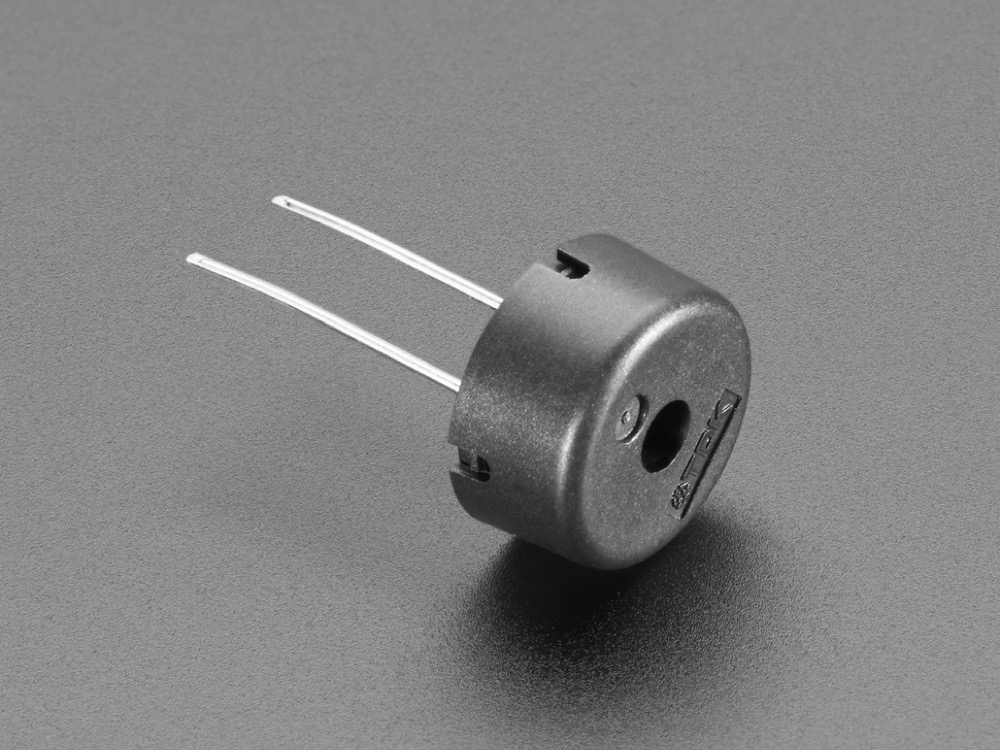
\includegraphics[width=0.75\linewidth,height=0.25\textheight,keepaspectratio]{images/materials-adafruit-buzzer.jpg}
  \caption{Buzzer}
  \caption*{Retrieved from \cite{website-materials-adafruit-buzzer}}
  \label{fig:materials-adafruit-buzzer}
\end{figure}

\subsection{LED}

This section requires no dependencies.

\begin{figure}[ht]
  \centering
  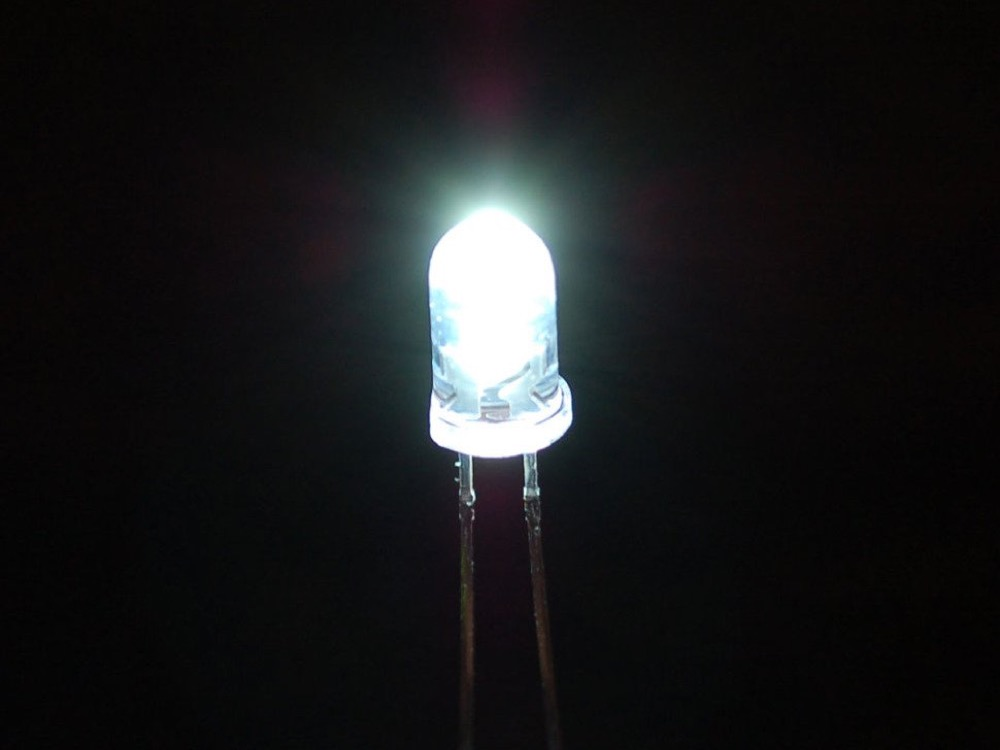
\includegraphics[width=0.75\linewidth,height=0.25\textheight,keepaspectratio]{images/materials-adafruit-led.jpg}
  \caption{LED}
  \caption*{Retrieved from \cite{website-materials-adafruit-led}}
  \label{fig:materials-adafruit-led}
\end{figure}

\subsection{MIDI}

We wrote functionalities to manipulate \acrshort{MIDI} instruments, and included examples to interface with some popular and cheap \acrshort{MIDI} instruments, such as the Korg volca beats.

We included examples for rhythmic and melodic elements, using two very ubiquitous and inexpensive \acrshort{MIDI} musical instruments, which are the Korg volca beats, and the Korg volca keys.

\begin{figure}[ht]
  \centering
  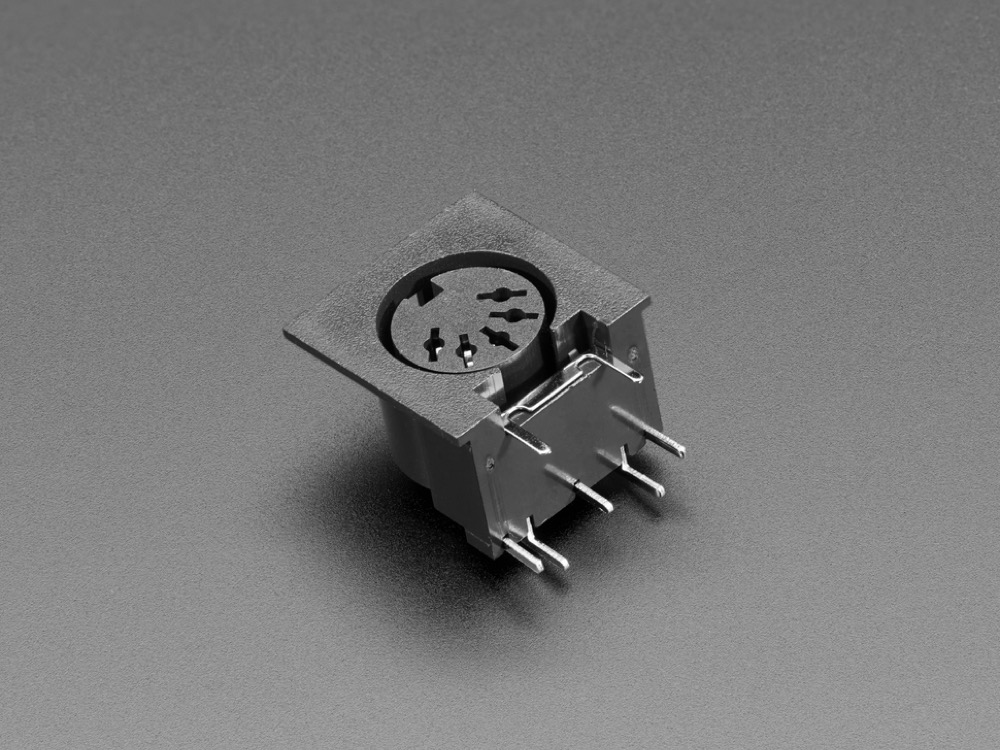
\includegraphics[width=0.75\linewidth,height=0.25\textheight,keepaspectratio]{images/materials-adafruit-midi-jack.jpg}
  \caption{MIDI jack}
  \caption*{Retrieved from \cite{website-materials-adafruit-midi-jack}}
  \label{fig:materials-adafruit-midi-jack}
\end{figure}

\subsection{Serial}

This output requires no library dependencies.

We use the already mentioned USB cable to connect to our computer, and receive messages over the serial port, available through the Arduino IDE.

\subsection{Screen}

This output requires a library for printing messages on a screen.

\begin{figure}[ht]
  \centering
  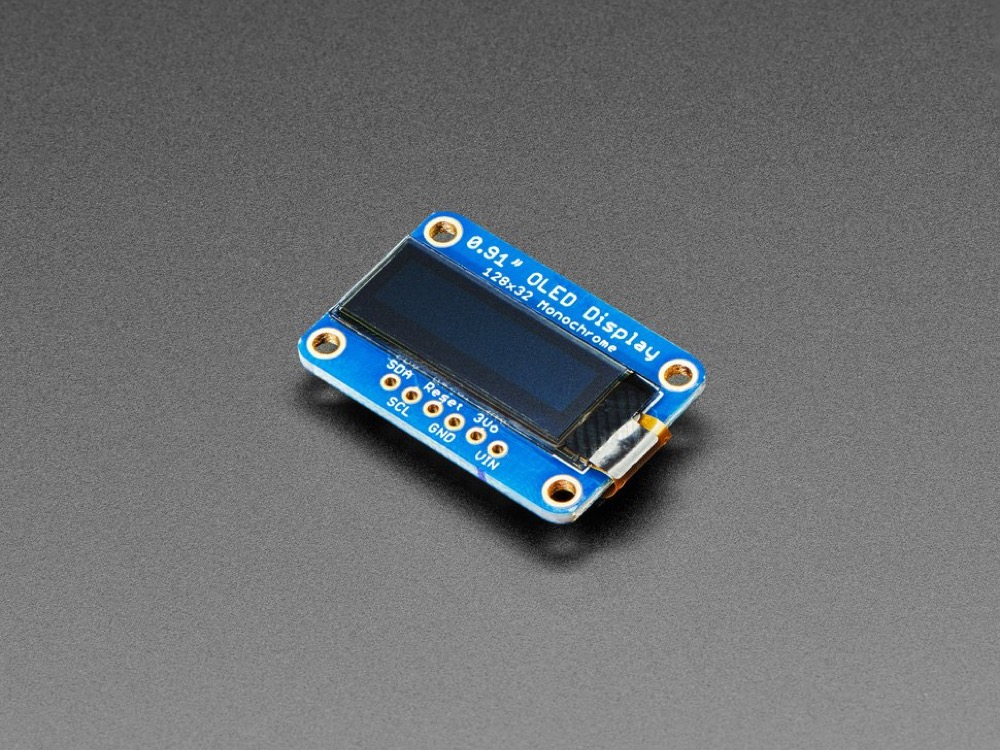
\includegraphics[width=0.75\linewidth,height=0.25\textheight,keepaspectratio]{images/materials-adafruit-screen.jpg}
  \caption{Screen}
  \caption*{Retrieved from \cite{website-materials-adafruit-screen}}
  \label{fig:materials-adafruit-screen}
\end{figure}

\subsection{Servo motor}

This output creates movement and through that, rhythmic sounds.

The main inspiration for this output was the emerging use of motor-activated percussive instruments, such as the Polyend Perc.

\begin{figure}[ht]
  \centering
  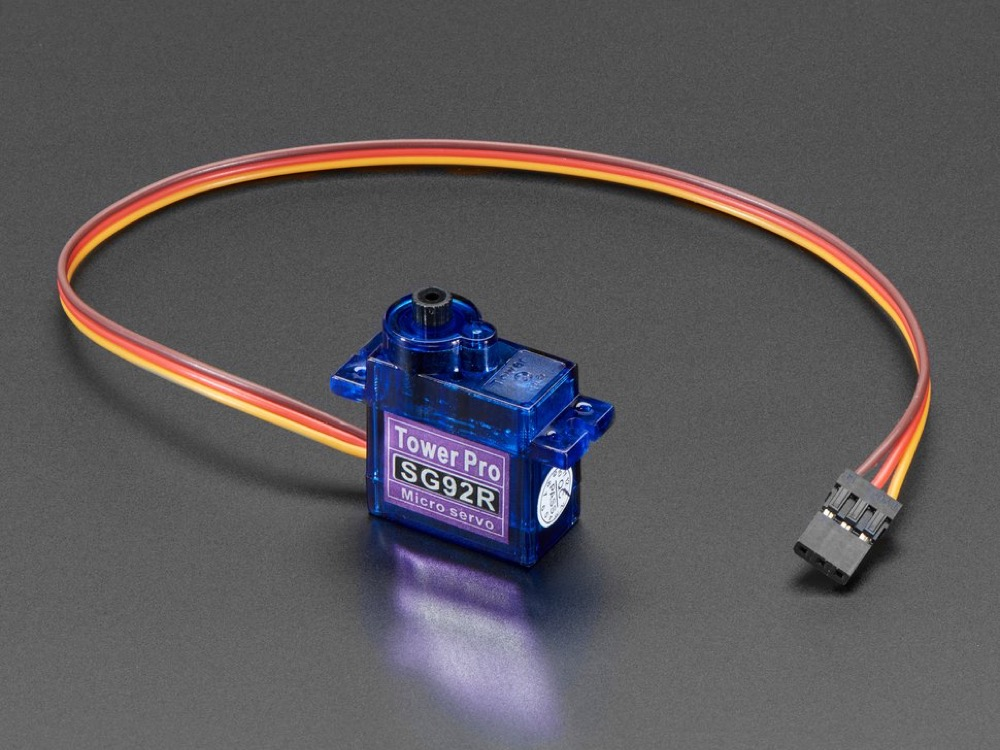
\includegraphics[width=0.75\linewidth,height=0.25\textheight,keepaspectratio]{images/materials-adafruit-servo.jpg}
  \caption{Micro servo motor}
  \caption*{Retrieved from \cite{website-materials-adafruit-servo}}
  \label{fig:materials-adafruit-servo}
\end{figure}

\subsection{Thermal printer}

A thermal printer is the basis for creating written and literary output, inspired by the field of computational poetry.

I used the popular Adafruit Thermal printer kit, which is documented on their website and includes a software library, distributed over GitHub and Arduino IDE, and also as a submodule on this project's TinyTrainable software library.

\begin{figure}[ht]
  \centering
  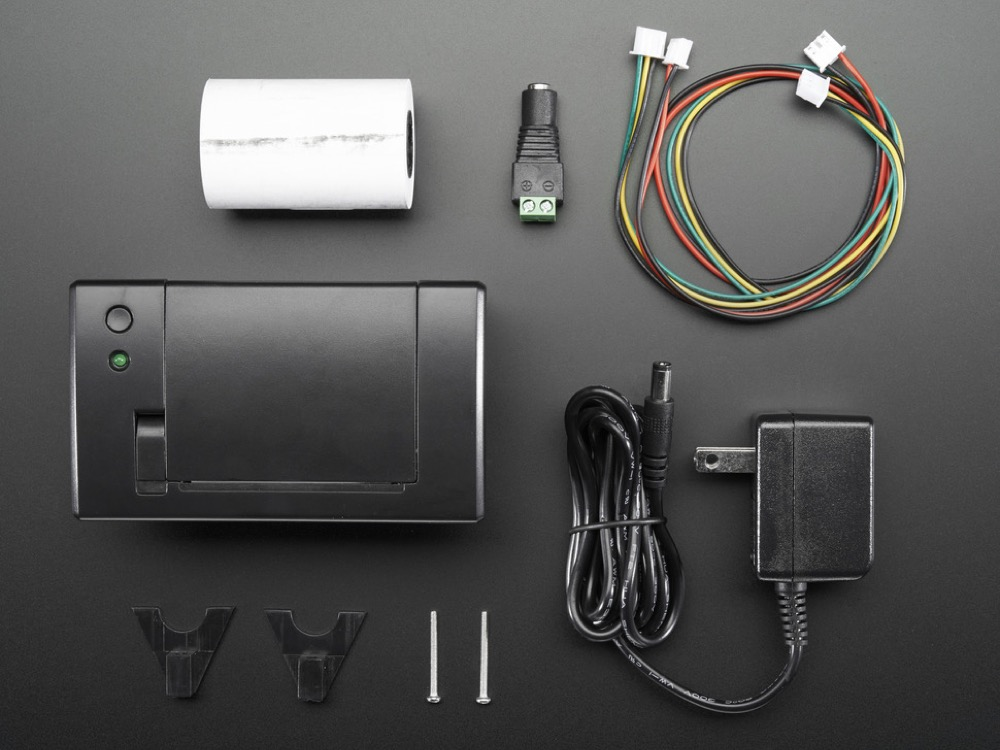
\includegraphics[width=0.75\linewidth,height=0.25\textheight,keepaspectratio]{images/materials-adafruit-thermal-printer.jpg}
  \caption{Thermal printer kit}
  \caption*{Retrieved from \cite{website-materials-adafruit-thermal-printer}}
  \label{fig:materials-adafruit-thermal-printer}
\end{figure}

\section{Development}

This thesis has been developed with the invaluable help of undergrad researchers Peter Tone and Maxwell Wang.

They have cloned both repositories, the main one and the Arduino library one, and have continuously submitted pull requests with their contributions.

Peter Tone has helped with research in data structures, library writing, and we have shared back and forth code, going from experimental proofs of concepts, and has also helped with the design of the user-facing library.

Maxwell Wang has proofread the code, has run the examples, and has helped with the writing of the documentation for self-learners and for the workshops.

We all share a Google Drive folder, where we all share notes about our research and development of the library and the educational material.

\section{Code}

This thesis is distributed as a repository, hosted on the GitHub platform, and available at https://github.com/montoyamoraga/tiny-trainable-instruments.

The auxiliary files, such as the LaTeX project for this document, and the auxiliary Jupyter notebooks, and documentation and tutorials are included on this repository.

The main software component of this project is the TinyTrainable library, available at https://github.com/montoyamoraga/TinyTrainable and also through the Arduino IDE.

The code included on this library is distributed on the folders:

\begin{enumerate}
  \item examples/
  \item src/
\end{enumerate}

\subsection{src/}

The source code for where there is a TinyTrainable.h and TinyTrainable.cpp file where we included all the basic functionality of the library. Additional subfolders include

\subsubsection{inputs/}

Base class Input and inherited classes for each one of the other inputs.

\subsubsection{outputs/}

Base class Output and inherited classes for each one of the other outputs.

\subsubsection{tensorflow/}

Auxiliary files, copied from the examples from the Arduino TensorFlow Lite that we are building on top of, and also from the newer TinyML library by the EdX team. These, unless otherwise noted, are included without modifications and distributed through the Apache License included on each file's headers.

\section{Tools}

This is a summary of tools used for making this project.

\subsection{clang-format}

Tool for automation of formatting to source code. More information at \url{https://clang.llvm.org/docs/.ClangFormat.html}.

\section{Doxygen}

Tool for generating documentation from the source code. More information at \url{https://www.doxygen.nl/}.

\subsection{GitHub Actions}

Every time we push code to the TinyTrainable repositories, a GitHub action creates a virtual machine, and runs a script to generate the Doxygen documentation and push it to the gh-pages branch, hosted at \url{https://montoyamoraga.github.io/TinyTrainable}.

\subsection{Jupyter}

Jupyter is a free, open-source browser application that allows users to easily read and write code in a clean, accessible environment. Code is segmented into cells, which users can run individually by clicking into and selecting the triangle "play" button at the top. Subsequent code runs based on operations done in previous cells. Basically, Jupyter notebooks allow programmers to create clean, step-by-step interactive walkthroughs through their code. More information at \url{https://jupyter-notebook-beginner-guide.readthedocs.io/en/latest/index.html}.
\subsection{Markdown}

Markdown is a lightweight markup language with simple, intuitive syntax. Aside from a few key differences, it is largely the same as plaintext. The documentation of this project is written using Markdown, including this document! More info at \url{https://guides.github.com/features/mastering-markdown/}
